\documentclass{beamer}

\usepackage[brazil]{babel}
\usepackage[utf8]{inputenc}

\usepackage{graphicx}
\usepackage{caption}
\usepackage{subcaption}

\usetheme{CambridgeUS}
\usecolortheme{dolphin}
\setbeamertemplate{blocks}[rounded][shadow=false]

\title[]{Multi-object Transportation using a Mobile Robot}
\author[Ramon Soares de Melo]{
Ramon Soares de Melo\\
Douglas G. Macharet\\
Mario Fernando Montenegro Campos
}
\institute[]
{
    
\includegraphics[height=0.1\textheight]{imgs/verlab.jpg}
    \hspace{0.4cm}
    
\includegraphics[height=0.1\textheight]{imgs/ppgcc.png}
    \hspace{0.4cm}
    
\includegraphics[height=0.1\textheight]{imgs/ufmg.png}\\
  % Instituto de Ciências Exatas - ICEx\\
  % Laboratório de Visão Computacional e Robótica - VerLab\\
  % Universidade Federal de Minas Gerais
}
\date{}
\subject{Computer Science}

\newcommand{\backupbegin}{
   \newcounter{framenumberappendix}
   \setcounter{framenumberappendix}{\value{framenumber}}
}
\newcommand{\backupend}{
   \addtocounter{framenumberappendix}{-\value{framenumber}}
   \addtocounter{framenumber}{\value{framenumberappendix}}
}

\begin{document}

    
\newcommand{\mrs}{MRS}
\newcommand{\environment}{\ensuremath{\mathbb{R}^3}}

% Shortcut definitions

\newcommand{\set}[1]{\ensuremath{\boldsymbol{\mathcal{#1}}}}
\newcommand{\setitem}[2]{\ensuremath{#1_{#2}}}
\newcommand{\setlist}[3]{#1\ $=$\ \{\setitem{#2}{1}, \setitem{#2}{2}, ..., \setitem{#2}{#3}\}}

\newcommand{\robotset}{\set{R}} % conjunto de robôs
\newcommand{\robotsetqt}{\ensuremath{k}}
\newcommand{\robot}[1]{\setitem{r}{#1}}
\newcommand{\robotlist}{\setlist{\robotset}{r}{\robotsetqt}}

\newcommand{\obstacleset}{\set{B}} % conjunto de obstáculos
\newcommand{\obstaclesetqt}{\ensuremath{x}}
\newcommand{\obstacle}[1]{\setitem{b}{#1}}
\newcommand{\obstaclelist}{\setlist{\obstacleset}{b}{\obstaclesetqt}}

\newcommand{\objectset}{\set{O}} % conjunto de objetos
\newcommand{\objectsetqt}{\ensuremath{y}}
\newcommand{\object}[1]{\setitem{o}{#1}}
\newcommand{\objectlist}{\setlist{\objectset}{o}{\objectsetqt}}

\newcommand{\planset}{\set{P}} % plano
\newcommand{\plansetqt}{\ensuremath{q}}
\newcommand{\plan}[1]{\setitem{n}{#1}}
\newcommand{\planlist}{\setlist{\planset}{n}{\plansetqt}}

\newcommand{\robotplanset}{\set{RP}} % conjunto de planos
\newcommand{\robotplansetqt}{\ensuremath{j}}
\newcommand{\robotplan}[1]{\setitem{rp}{#1}}
\newcommand{\robotplanlist}{\setlist{\robotplanset}{rp}{\robotplansetqt}}

\newcommand{\executionplanset}{\set{EP}} % conjunto de planos
\newcommand{\executionplansetqt}{\ensuremath{h}}
\newcommand{\executionplan}[1]{\setitem{ep}{#1}}
\newcommand{\executionplanlist}{\setlist{\executionplanset}{ep}{\executionplansetqt}}
\newcommand{\executionplanname}{\emph{Execution Plan}}
\newcommand{\executionplansetnotation}{\ensuremath{\executionplanset \subset \robotplanset}}

\newcommand{\executionplanminset}{\ensuremath{\executionplanset{*}}} % conjunto com custo minimo de segmentos

\newcommand{\segmentset}{\set{S}} % conjunto de segmentos
\newcommand{\segmentsetqt}{\ensuremath{e}}
\newcommand{\segment}[1]{\setitem{s}{#1}}
\newcommand{\segmentlist}{\setlist{\segmentset}{s}{\segmentsetqt}}

\newcommand{\segmentpointset}{\ensuremath{\set{S}_p}} % conjunto de pontos de segmentação
\newcommand{\segmentpointsetqt}{\ensuremath{z}}
\newcommand{\segmentpoint}[1]{\setitem{sp}{#1}}
\newcommand{\segmentpointfirst}[1]{\ensuremath{\segmentpoint{#1}^1}}
\newcommand{\segmentpointsecond}[1]{\ensuremath{\segmentpoint{#1}^2}}

\newcommand{\segmentpointlist}{\setlist{\segmentpointset}{sp}{\segmentpointsetqt}}

\newcommand{\typeland}{ground}
\newcommand{\typeaerial}{aerial}
\newcommand{\typeset}{\set{T}} % conjunto de tipos de movimentação
\newcommand{\typelist}{\ensuremath{\typeset=\ \{}\typeland, \typeaerial\ensuremath{\}}}
\newcommand{\type}[1]{\setitem{t}{#1}}

\newcommand{\plantypestart}{initial}
\newcommand{\plantypetransition}{transition}
\newcommand{\plantypemove}{movement}
\newcommand{\plantypeset}{\set{TP}} % conjunto de tipos de plano
\newcommand{\plantypelist}{\ensuremath{\plantypeset=\ \{}\plantypestart, \plantypetransition, \plantypemove\ensuremath{\}}}
\newcommand{\plantype}[1]{\setitem{tp}{#1}}

\newcommand{\movementtypepremove}{pre-transport}
\newcommand{\movementtypemove}{transport}
\newcommand{\movementtypeset}{\set{T_m}} % conjunto de tipos de plano
\newcommand{\movementtypelist}{\ensuremath{\movementtypeset=\ \{}\movementtypepremove, \movementtypemove\ensuremath{\}}}
\newcommand{\movementtype}[1]{\setitem{tm}{#1}}

\newcommand{\tokenset}{\set{TO}}
\newcommand{\tokensetqt}{\ensuremath{u}}
\newcommand{\tokeni}[1]{\setitem{to}{#1}}
\newcommand{\token}{\emph{token}}
\newcommand{\tokenlist}{\setlist{\tokenset}{to}{\tokensetqt}}

\newcommand{\workspace2}{\ensuremath{\boldsymbol{\mathcal{W}}}} % àrea de trabalho
\newcommand{\workspacecell}{\ensuremath{\boldsymbol{\mathcal{c}}}} % àrea de trabalho

\newcommand{\allocationgraph}{\ensuremath{\mathcal{AG}}}
\newcommand{\allocationgraphcompress}{\ensuremath{\mathcal{AG}_c}}

\newcommand{\currentstate}{\ensuremath{S}}
\newcommand{\nextstate}{\ensuremath{S'}}
\newcommand{\originstate}{\ensuremath{S_o}}
\newcommand{\targetstate}{\ensuremath{S_d}}
\newcommand{\robotstate}{\ensuremath{S_r}}

\newcommand{\robotinitialstate}{\ensuremath{I}}
\newcommand{\robotinitialstatei}[1]{\ensuremath{I_{#1}}}

\newcommand{\celldimension}{\ensuremath{d}}
\newcommand{\deslocationfactor}{\ensuremath{l}}

\newcommand{\movementset}{\set{M}}
\newcommand{\movementslist}{\ensuremath{\movementset=\ \{}left, right, front, back, up, down\ensuremath{\}}}
\newcommand{\movementaction}{\ensuremath{a_i}}

% Funções

\newcommand{\utilityfunction}{\ensuremath{\Theta}}
\newcommand{\utilityplanfunction}{\ensuremath{\utilityfunction_{p}}}
\newcommand{\utilitytotalfunction}{\ensuremath{\utilityfunction_{t}}}
\newcommand{\distancefunction}{\ensuremath{\Delta}}
\newcommand{\timefunction}{\ensuremath{\Upsilon}}
\newcommand{\energyfunction}{\ensuremath{\Psi}}

% Planejamento

\newcommand{\fringe}{\set{F}}
\newcommand{\searchednodes}{\set{SN}}
\newcommand{\node}{\ensuremath{n}}
\newcommand{\nodeitem}[1]{\ensuremath{\node_{#1}}}
\newcommand{\nodeparent}{\emph{NodePai}}
\newcommand{\nodeutility}{\ensuremath{\omega}}
\newcommand{\nodedata}{\ensuremath{\{}state (\currentstate), action (\movementaction), utility (\nodeutility), agent's position (\robotstate), type (\type{i})\ensuremath{\}}}


    \frame{
        \titlepage
    }

    \section{Introduction} % (fold)

    \subsection{Motivation} % (fold)
    % \label{sub:motiva_o}

    \frame{
        \frametitle{Object Manipulation}

        Transport and manipulation of objects is a basic task in other actions:

        \begin{figure}[p]

            \centering
            \begin{subfigure}[b]{0.24\textwidth}
                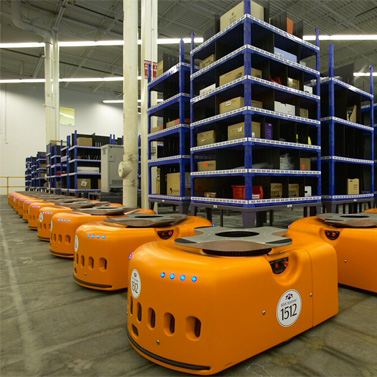
\includegraphics[width=\textwidth]{imgs/transporte1.png}
                \caption*{Transport}
            \end{subfigure}
            \begin{subfigure}[b]{0.24\textwidth}
                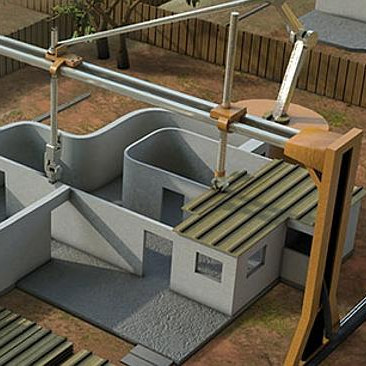
\includegraphics[width=\textwidth]{imgs/transporte2.jpg}
                \caption*{Construction}
            \end{subfigure}
            \begin{subfigure}[b]{0.24\textwidth}
                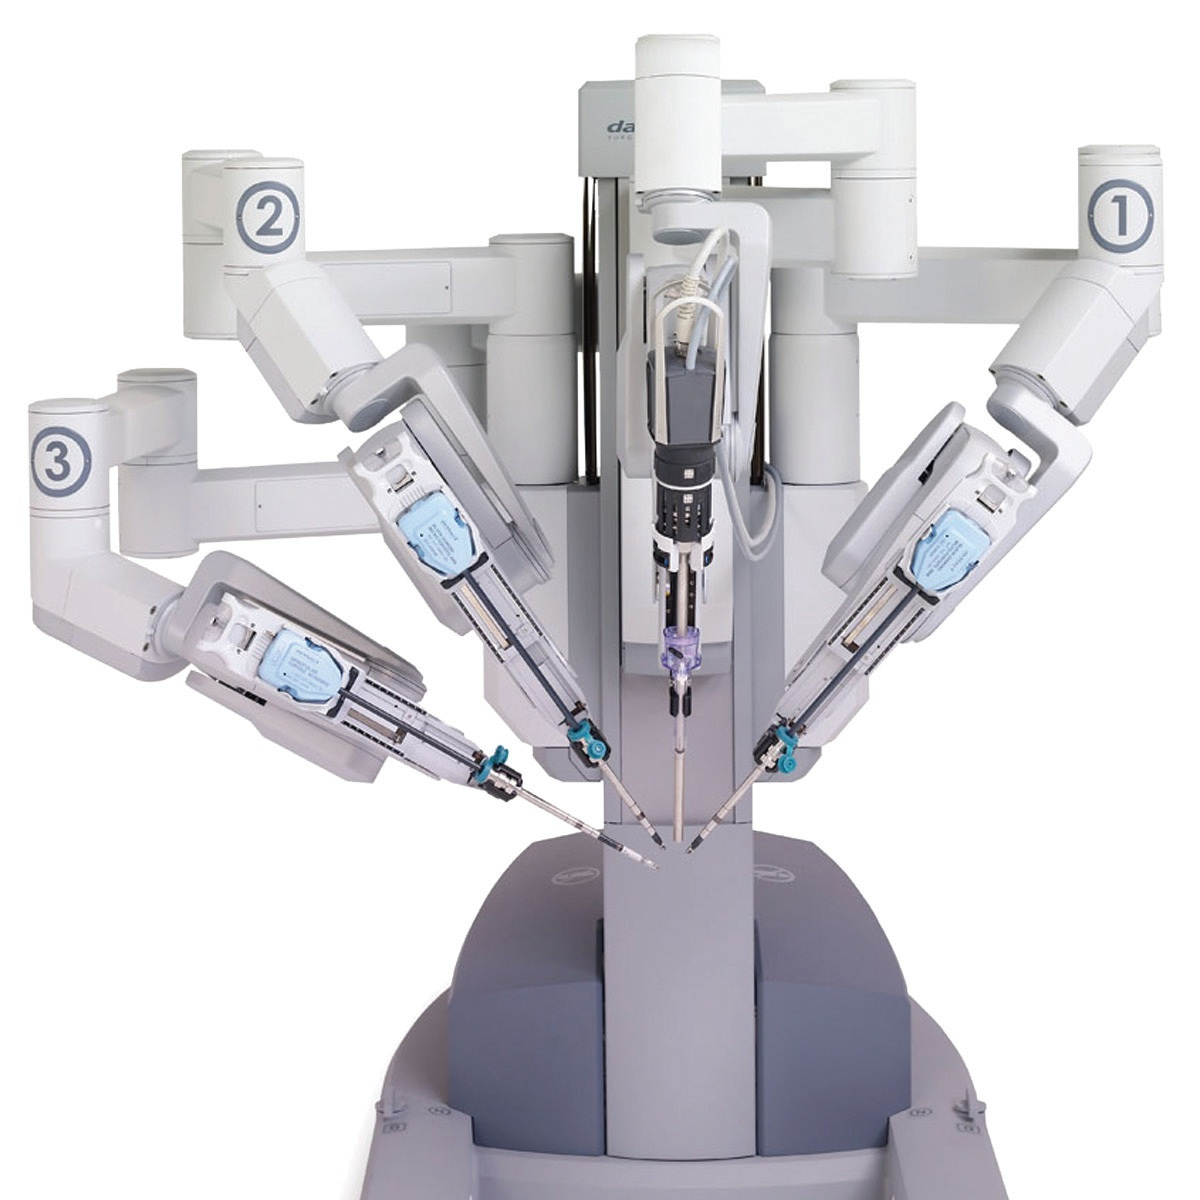
\includegraphics[width=\textwidth]{imgs/transporte3.jpg}
                \caption*{Tools}
            \end{subfigure}
            \begin{subfigure}[b]{0.24\textwidth}
                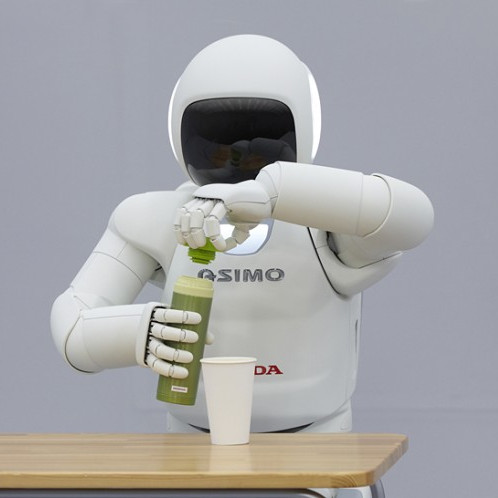
\includegraphics[width=\textwidth]{imgs/transporte4.jpg}
                \caption*{Household Usage}
            \end{subfigure}

        \end{figure}
    }

    \frame{
        \frametitle{Types of manipulation}

        \begin{columns}[T]
            \begin{column}[T]{0.5\textwidth}

                \begin{block}{Prehensile}
                    Agent uses a manipulator to hold the object to be transported.
                \end{block}

                \begin{figure}[p]
                    \centering
                    \setlength{\fboxsep}{0pt}
                    \fbox{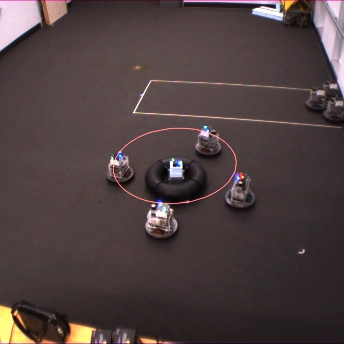
\includegraphics[width=0.6\textwidth]{imgs/fink.png}}
                    \caption*{\cite{Fink2008}}
                \end{figure}

            \end{column}
            \begin{column}[T]{0.5\textwidth}

                \begin{block}{Non-prehensile}
                    Agent uses action like trowing, rolling or pushing to transport the object.
                \end{block}

                \begin{figure}[p]
                    \centering
                    \setlength{\fboxsep}{0pt}
                    \fbox{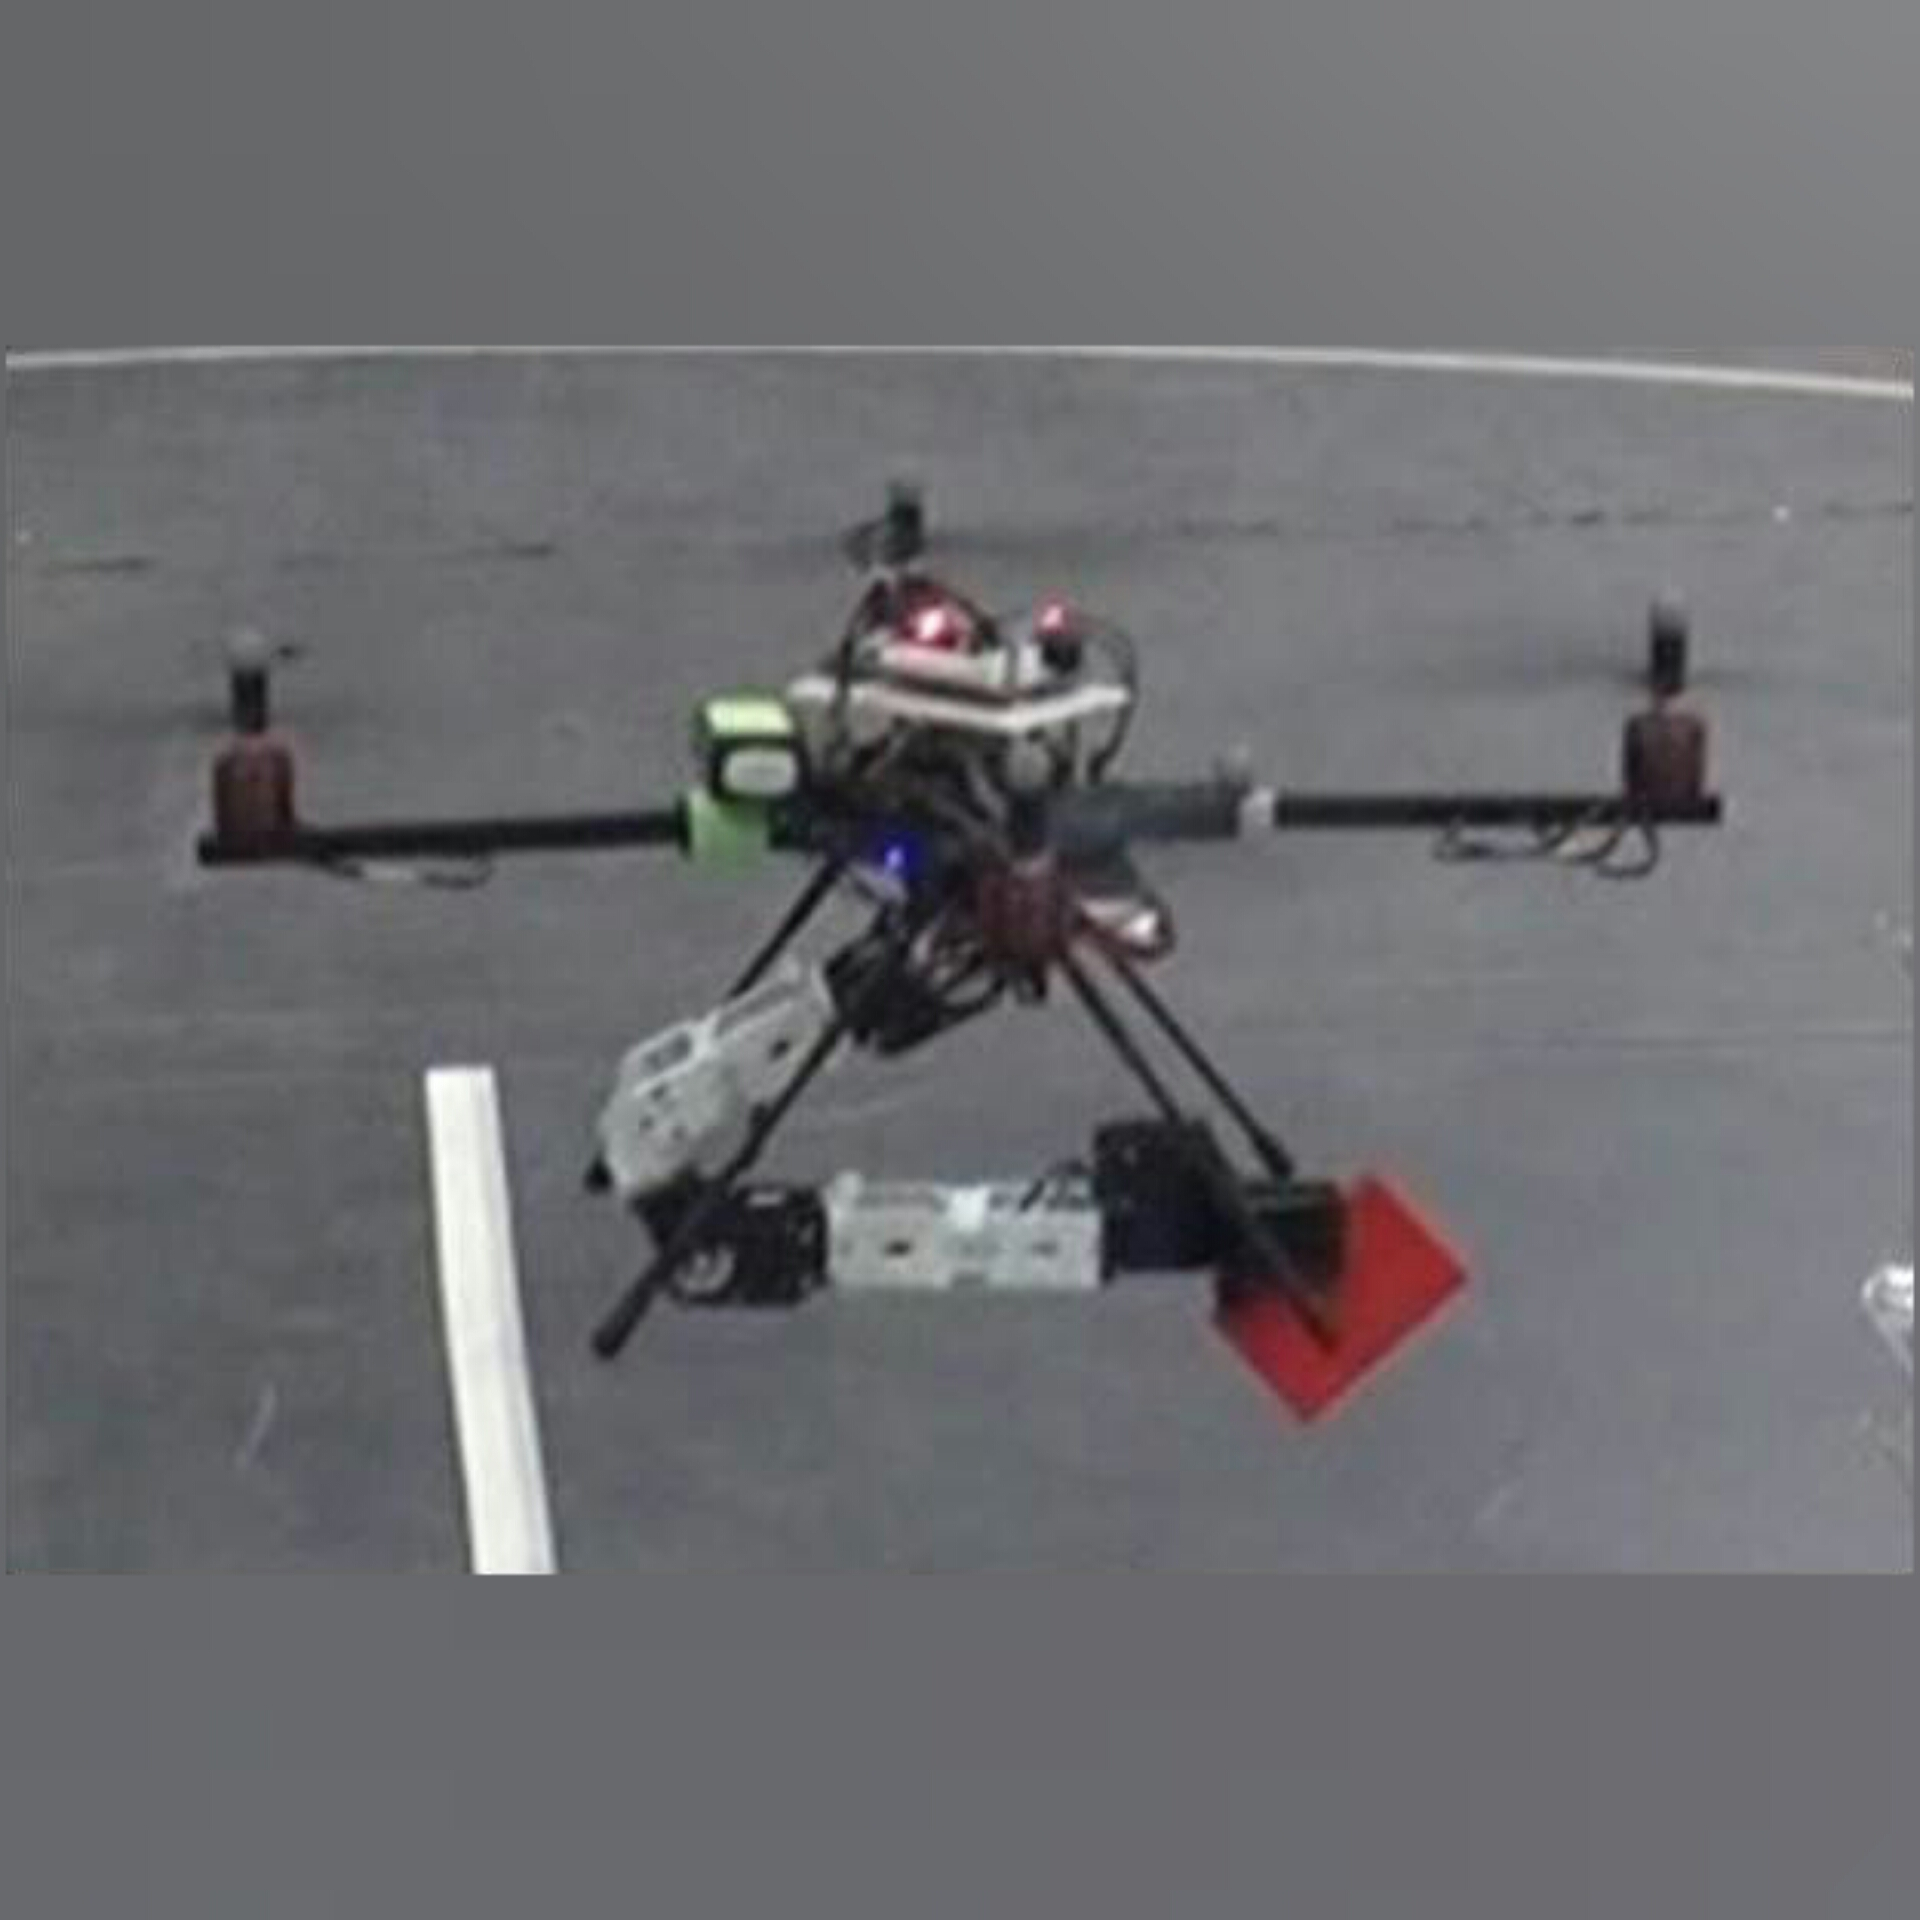
\includegraphics[width=0.6\textwidth]{imgs/kim.png}}
                    \caption*{\cite{Kim2013}}
                \end{figure}

            \end{column}
        \end{columns}
    }

    \section{Related Works}

    \frame{
        \frametitle{Related Works}

        \begin{itemize}
            \item Inoue, Reiko, et al. "Rearrangement of multiple objects by a robot group having a multi-task function." International Conference on Robotics and Biomimetics 2009.
            \vspace{0.4cm}
            % Two types of robots, the single-function and multi-function
            % Studies how to schedule and plan a sequence of transports
            % using this robots
            \item Behrens, Michael, et al. "Models for pushing objects with a mobile robot using single point contact." International Conference on Intelligent Robots and Systems (IROS) 2010.
            \vspace{0.4cm}
            % Presents a mathematical model for pushing objects based only
            % one contact point, which is necessary in cases when objects
            % can not be grasped
            \item Shiroma, Pedro M., and Mario FM Campos. "CoMutaR: A framework for multi-robot coordination and task allocation." International Conference on Intelligent Robots and Systems (IROS) 2009.
            % Describes a method to allocate tasks and coordinate agents.
            % The tasks are divided into atomic parts, called actions,
            % The execution of each action results on the realization of the mission
        \end{itemize}

    }

    \section{Methodology}
    \subsection{Problem} % (fold)

    \frame{
        \frametitle{Problem Definition}

        \begin{columns}[c, onlytextwidth]
            \begin{column}[c]{0.6\textwidth}

                Workspace know and discrete, with the following groups:

                \begin{itemize}
                    \item Objects to be transported;
                    \item Obstacles, blocking objects;
                    \item Agent.
                \end{itemize}

            \end{column}
            \begin{column}[c]{0.35\textwidth}
                \begin{figure}[p]
                    \centering
                    \setlength{\fboxsep}{0pt}
                    \fbox{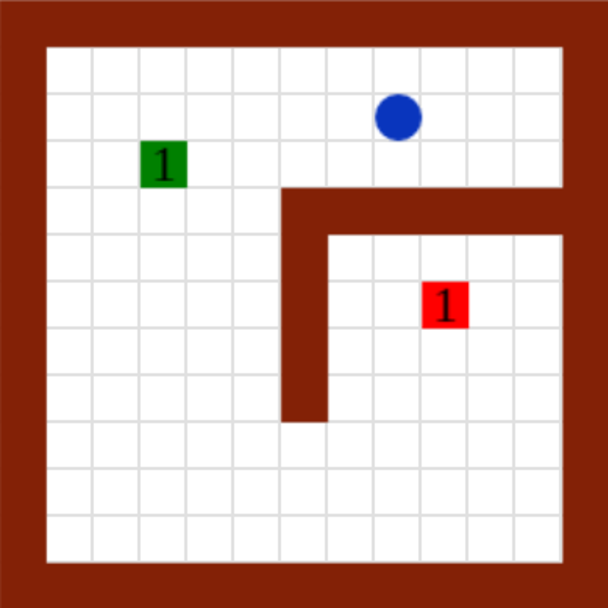
\includegraphics[width=0.95\textwidth]{imgs/MoveIntro_0.pdf}}
                    \caption*{\centering Workspace}
                \end{figure}
            \end{column}
        \end{columns}
    }

    \frame{
        \frametitle{Problem Definition}

        \begin{columns}[c]
          \begin{column}{0.7\textwidth}

            \textbf{Problem 1} \textit{Object Path Planning}
            \vspace{0.2cm}\\
            Find a feasible path inside the workspace to each object, starting from its initial position until a desired end position.

          \end{column}
          \begin{column}{0.3\textwidth}
            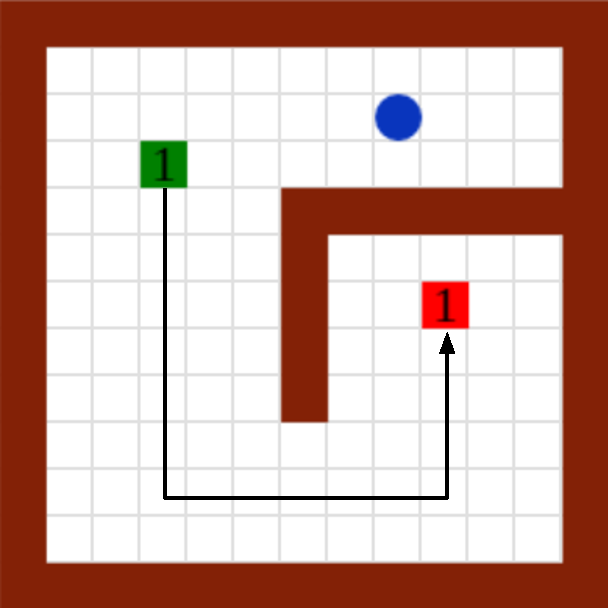
\includegraphics[width=\textwidth]{imgs/MoveIntro_1.pdf}
          \end{column}
        \end{columns}

        \begin{columns}[c]
          \begin{column}{0.7\textwidth}

            \textbf{Problem 2} \textit{Task Allocation and Execution}
            \vspace{0.2cm}\\
            Control the agent to create a set of plans to accomplish all tasks, trying to minimize the total traveled distance.

          \end{column}
          \begin{column}{0.3\textwidth}
            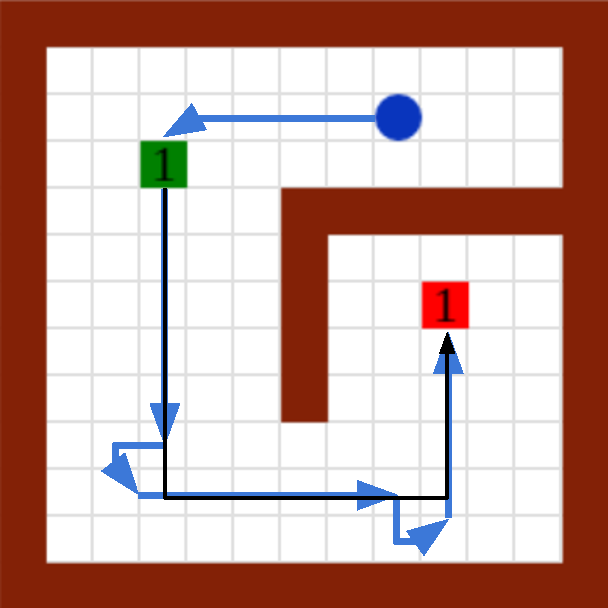
\includegraphics[width=\textwidth]{imgs/MoveIntro_2.pdf}
          \end{column}
        \end{columns}
    }

    \frame{
        \frametitle{Path Planning - Object}

        \begin{columns}[c]

            \begin{column}[c]{0.5\textwidth}
                Planning for a object from set \objectset\ has two phases:

                \begin{enumerate}
                    \item \emph{Planning}: a travel plan is created;
                    \vspace{0.2cm}
                    \item \emph{Segmentation}: the plan is splitted into sub-plans.
                \end{enumerate}
            \end{column}

            \begin{column}[c]{0.5\textwidth}
                \begin{figure}[p]
                    \centering
                    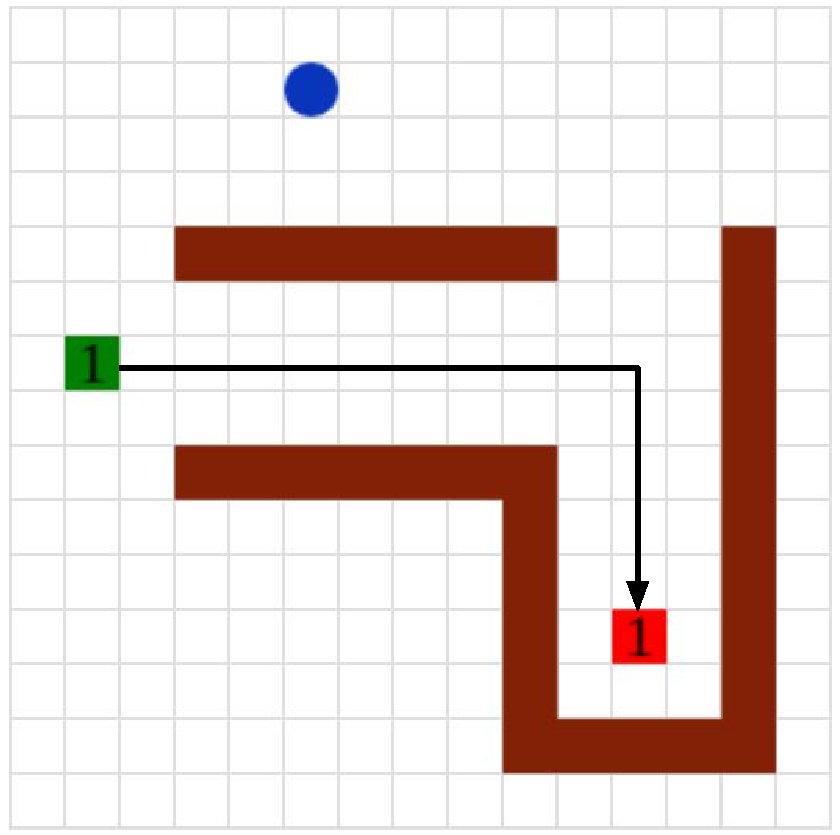
\includegraphics[width=0.9\textwidth]{imgs/ObjectPlanning.pdf}
                    \caption*{Object Plan}
                \end{figure}
            \end{column}

        \end{columns}
    }

    \frame{
        \frametitle{Path Planning - Object}
        \framesubtitle{Planning Algorithm}

        \begin{block}{Description}
            \begin{itemize}
                \item Based on A* Algorithm;
                \item Using as Heuristic the remainder distance to the goal.
            \end{itemize}
        \end{block}

        \begin{figure}[p]

            \centering
            \begin{subfigure}[b]{0.3\textwidth}
                \fbox{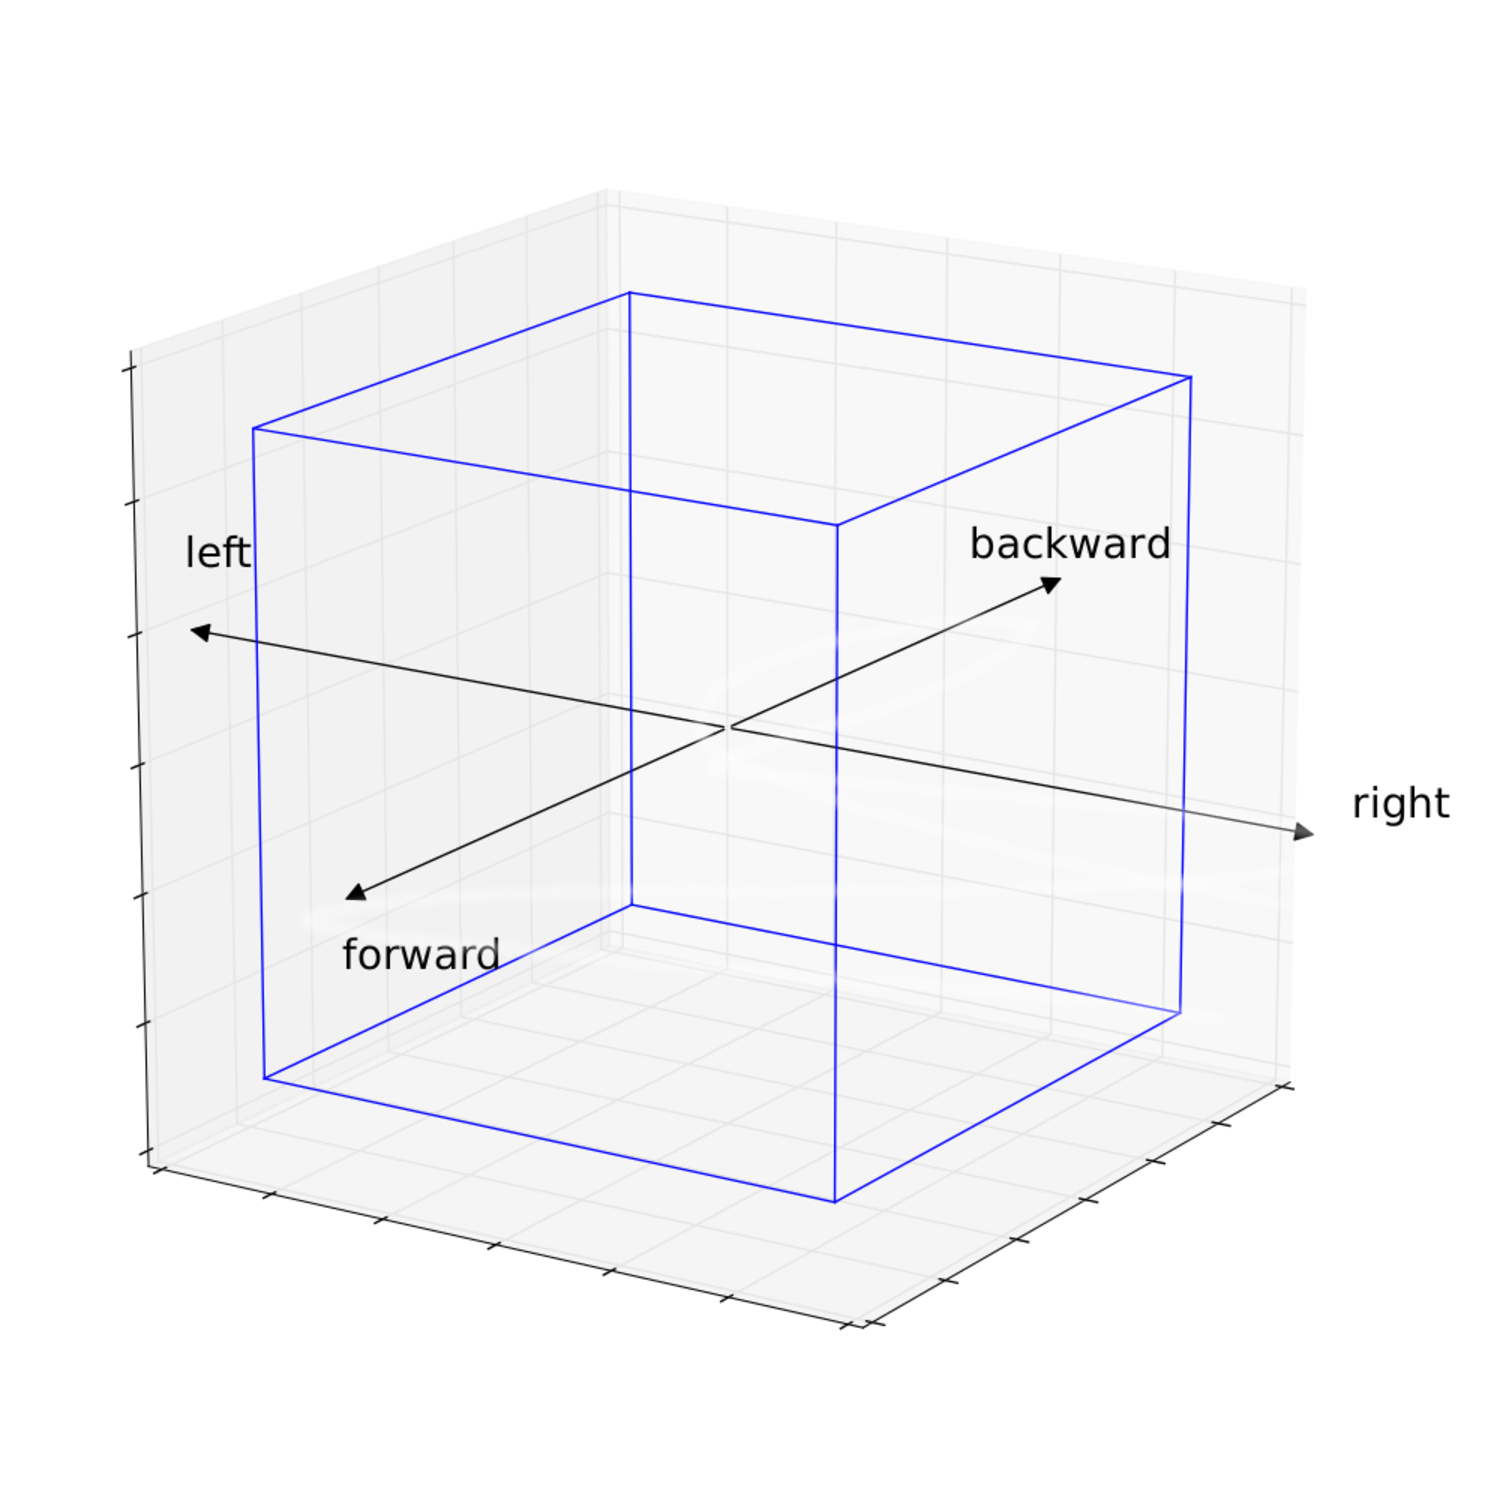
\includegraphics[width=\textwidth]{imgs/movements.pdf}}
                \caption*{Available movements.}
            \end{subfigure}
            \hspace{0.5cm}
            \begin{subfigure}[b]{0.3\textwidth}
                \fbox{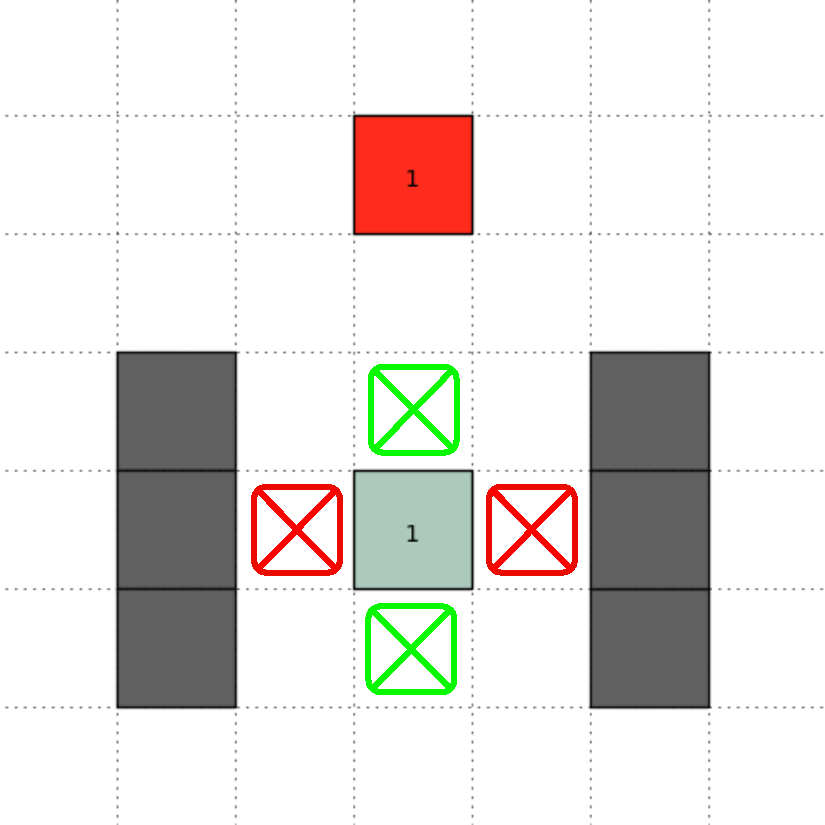
\includegraphics[width=\textwidth]{imgs/teste1.pdf}}
                \caption*{Collision test.}
            \end{subfigure}

        \end{figure}
    }

    \frame{
        \frametitle{Path Planning - Object}
        \framesubtitle{Segmentation Algorithm}

        \begin{columns}[c]

            \begin{column}[c]{0.5\textwidth}
                Segmentation occurs in two steps:

                \begin{enumerate}
                    \item Creation of segmentation points;
                    \item Plan segmentation.
                \end{enumerate}
            \end{column}

            \begin{column}[c]{0.5\textwidth}
                \begin{figure}[p]
                    \centering
                    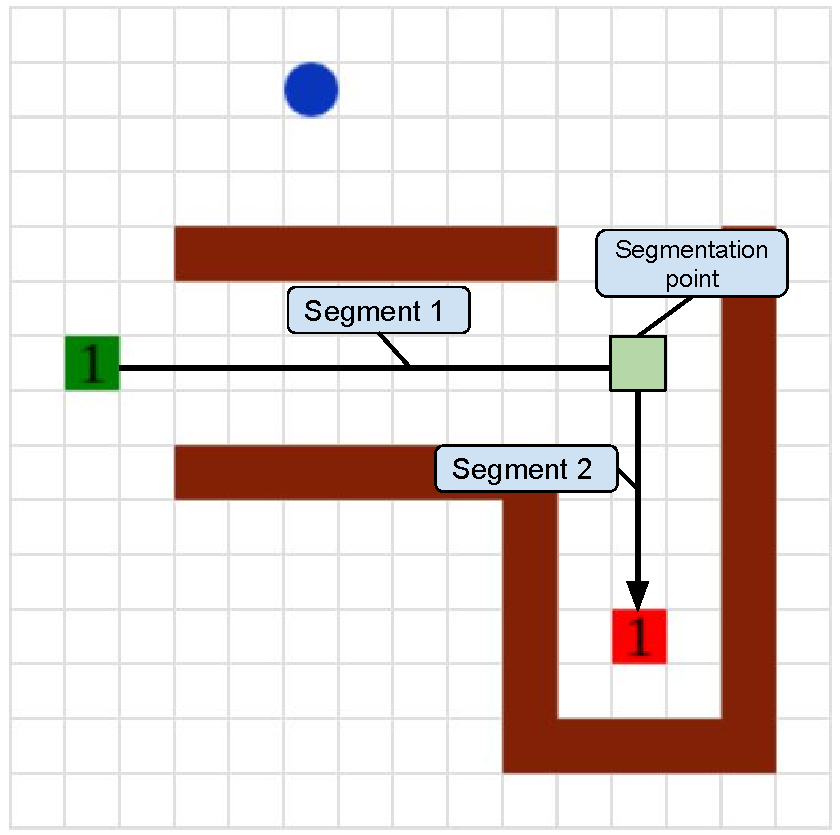
\includegraphics[width=0.9\textwidth]{imgs/ObjectSegmentation.pdf}
                    \caption*{Object Plan segmented}
                \end{figure}
            \end{column}

        \end{columns}
    }

    \frame{
        \frametitle{Path Planning - Agents}

        \begin{columns}[c]

            \begin{column}[c]{0.5\textwidth}
                Based on segments created from the object's plan, movimentation plans are created, of two types:

                \begin{itemize}
                    \item \emph{Preparation}: plan in which the robot approaches the object to be transported;
                    \vspace{0.2cm}
                    \item \emph{Transport}: plan used to transport the object.
                \end{itemize}
            \end{column}

            \begin{column}[c]{0.5\textwidth}
                \begin{figure}[p]
                    \centering
                    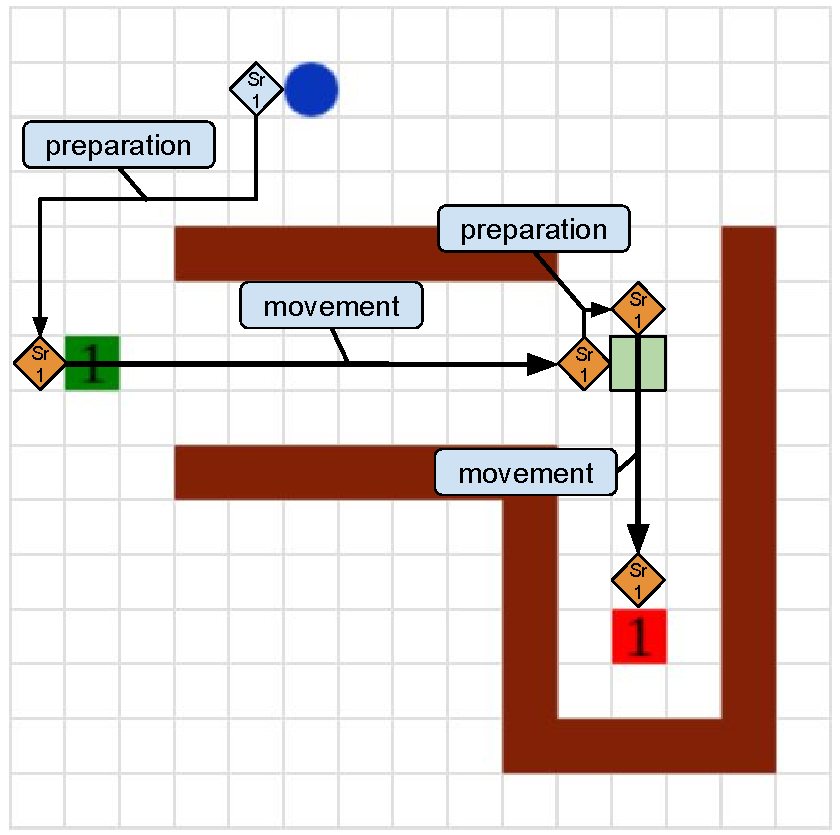
\includegraphics[width=0.9\textwidth]{imgs/ObjectRobotPlans.pdf}
                    \caption*{Agent's Plan}
                \end{figure}
            \end{column}

        \end{columns}
    }

    \frame{
        \frametitle{Task Allocation}

        \begin{figure}[p]
            \centering
            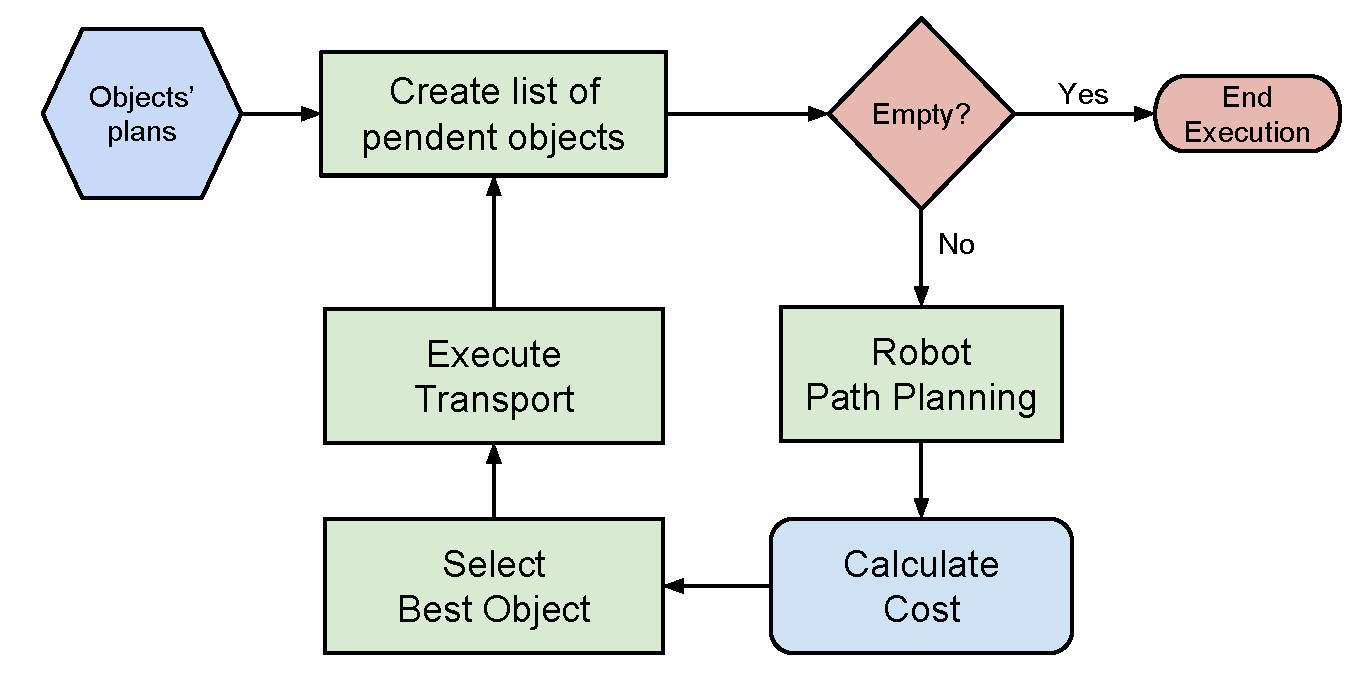
\includegraphics[width=0.9\textwidth]{imgs/TaskAllocationSingleRobot.pdf}
            \caption*{Task Allocation Process}
        \end{figure}
    }

    \frame{
        \frametitle{Task Allocation}

        \begin{block}{Execution Example}
            \begin{figure}[p]
                \centering
                \begin{subfigure}[b]{0.24\textwidth}
                    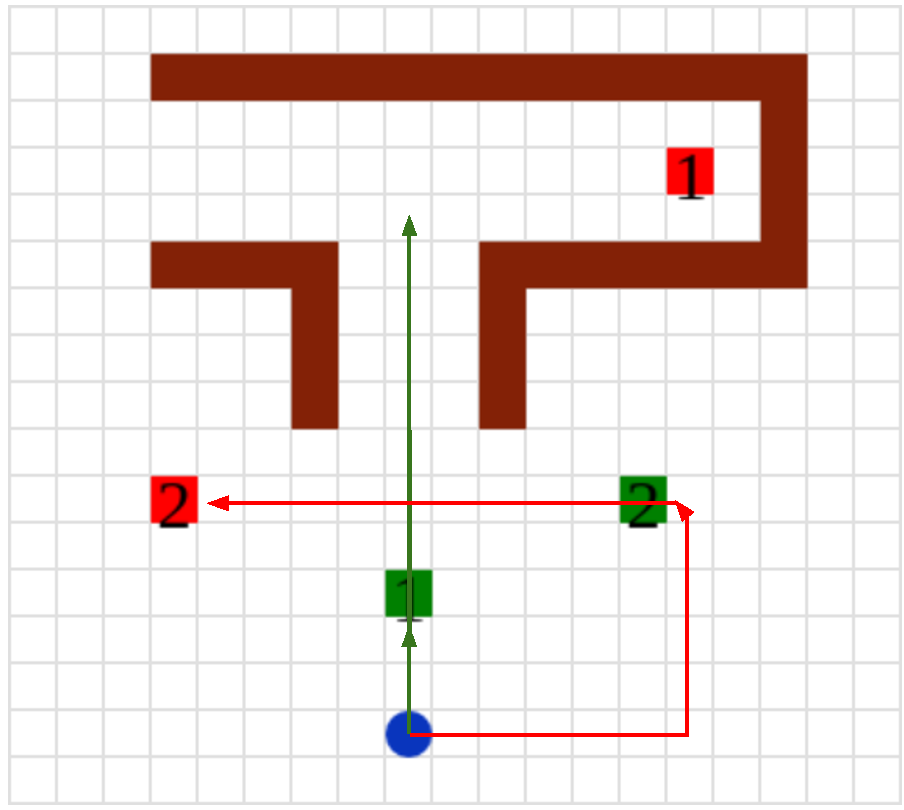
\includegraphics[width=\textwidth]{imgs/coordination/Mov1.pdf}
                    \caption*{Select Object 1}
                \end{subfigure}
                \begin{subfigure}[b]{0.24\textwidth}
                    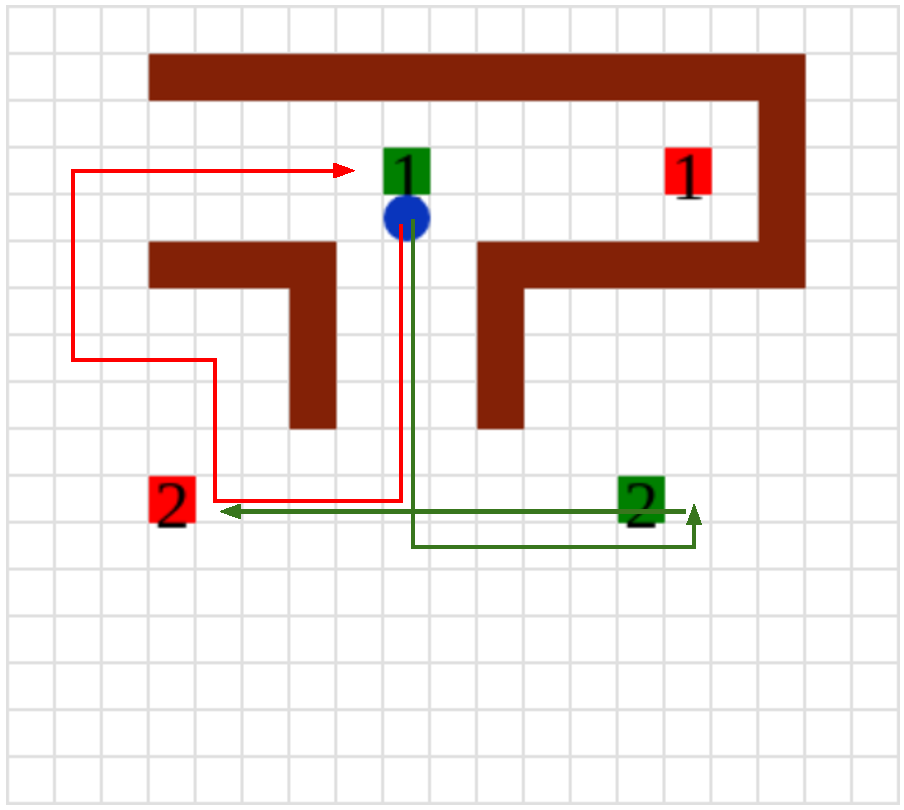
\includegraphics[width=\textwidth]{imgs/coordination/Mov2.pdf}
                    \caption*{Select Object 2}
                \end{subfigure}
                \begin{subfigure}[b]{0.24\textwidth}
                    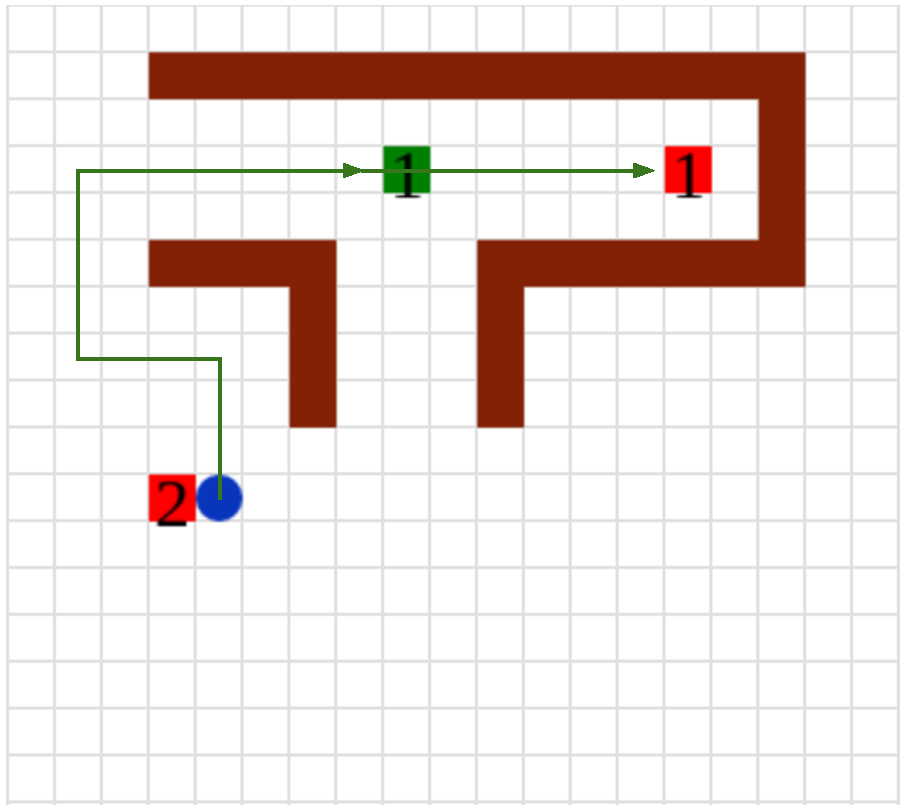
\includegraphics[width=\textwidth]{imgs/coordination/Mov3.pdf}
                    \caption*{Select Object 1}
                \end{subfigure}
                \begin{subfigure}[b]{0.24\textwidth}
                    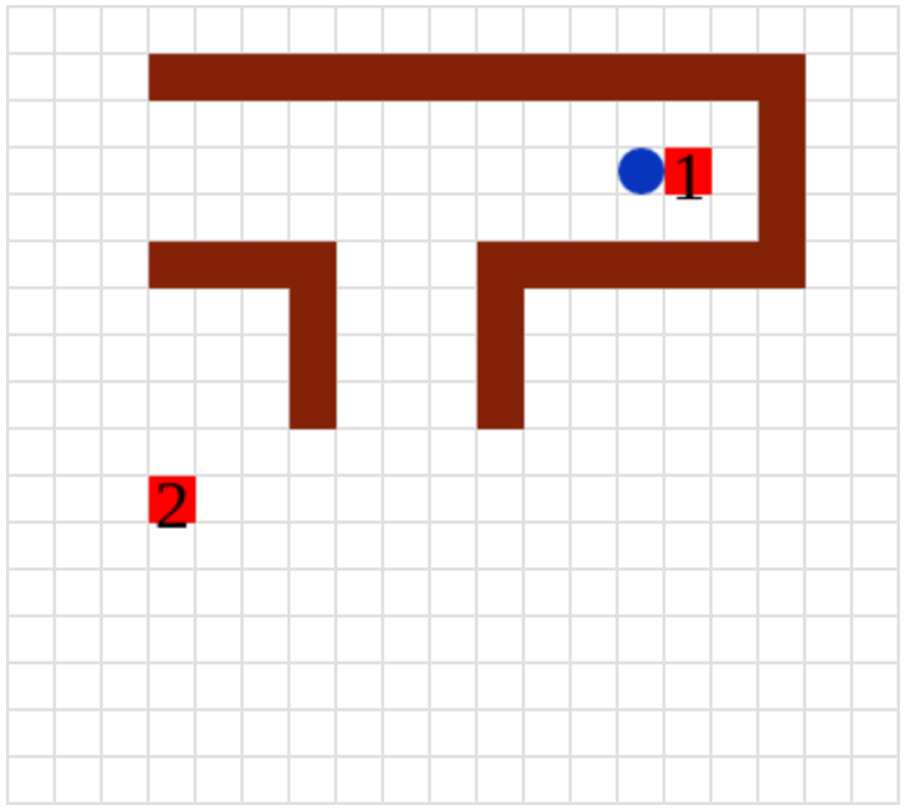
\includegraphics[width=\textwidth]{imgs/coordination/Mov4.pdf}
                    \caption*{Completed}
                \end{subfigure}
            \end{figure}
        \end{block}
    }

    \section{Experiments} % (fold)

    \frame{
        \frametitle{Experiments}

        \begin{block}{Description}
            The proposed methodology was compared with a simple transportation method, in which transport of objects is made in a sequential manner.

            \vspace{0.2cm}
            Several tests were conducted to examine the methods behavior, considering two types:
            \begin{enumerate}
                \item Total time of planning and task allocation phases;
                \item Sum of total traveled space in unit cells by the agent;
            \end{enumerate}
        \end{block}
    }

    \frame{
        \frametitle{Experiments}

        \begin{block}{Illustrative Comparison}
            \begin{figure}[p]
                \centering
                \begin{subfigure}[b]{0.48\textwidth}
                    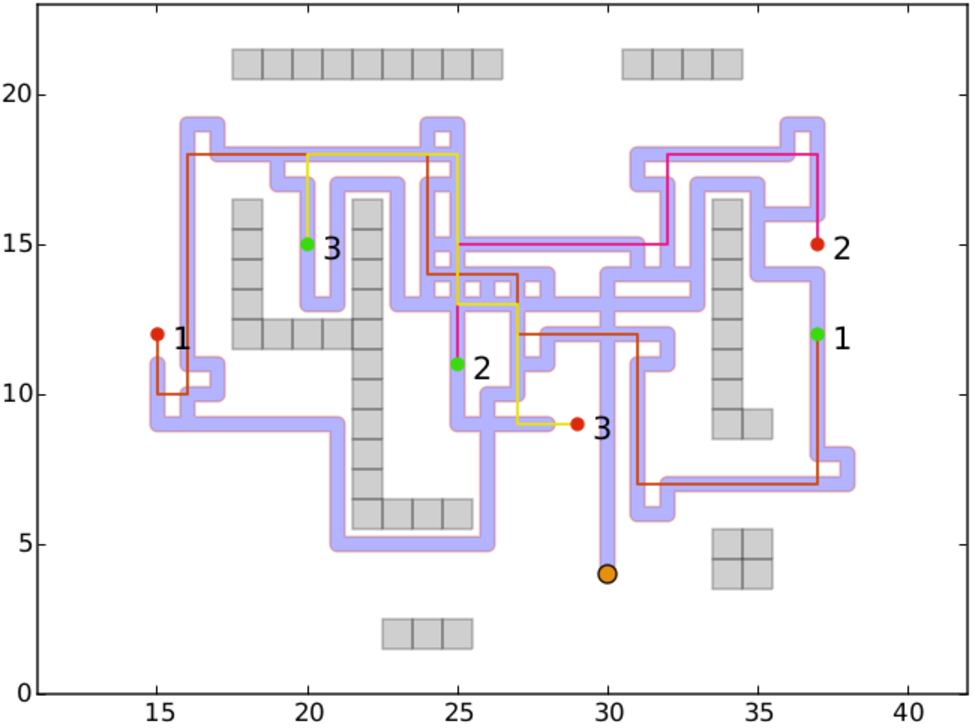
\includegraphics[width=\textwidth]{imgs/path_basic_method.pdf}
                    \caption*{Sequential Method}
                \end{subfigure}
                \begin{subfigure}[b]{0.48\textwidth}
                    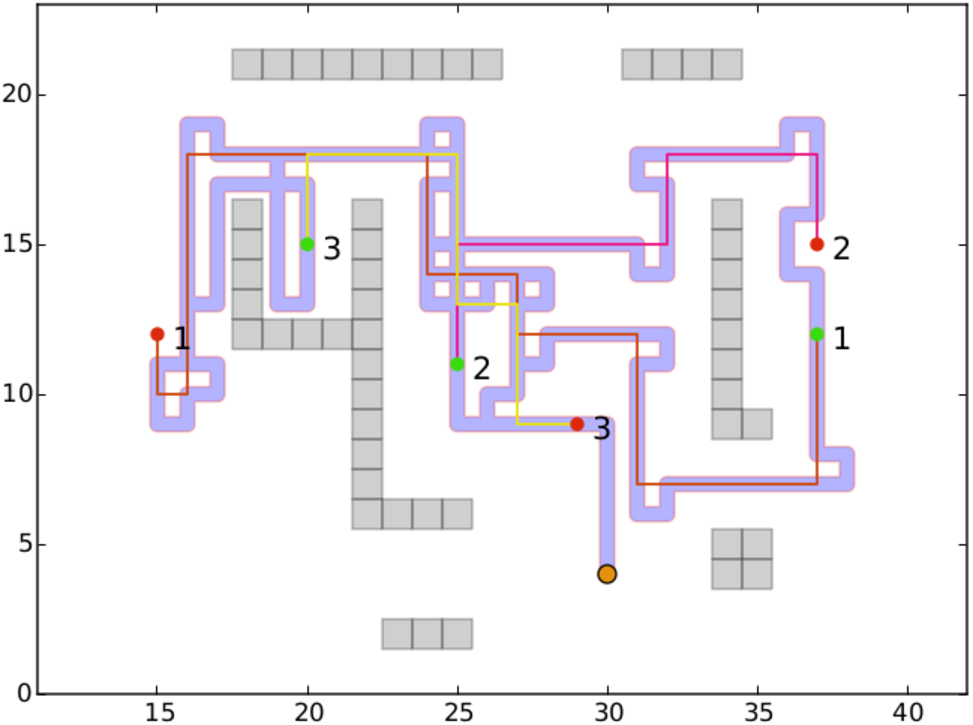
\includegraphics[width=\textwidth]{imgs/path_proposed_method.pdf}
                    \caption*{Proposed Method}
                \end{subfigure}
            \end{figure}
        \end{block}
    }

    \frame{
        \frametitle{Experiments}

        \begin{block}{Planning Time}
            \begin{figure}[p]
                \centering
                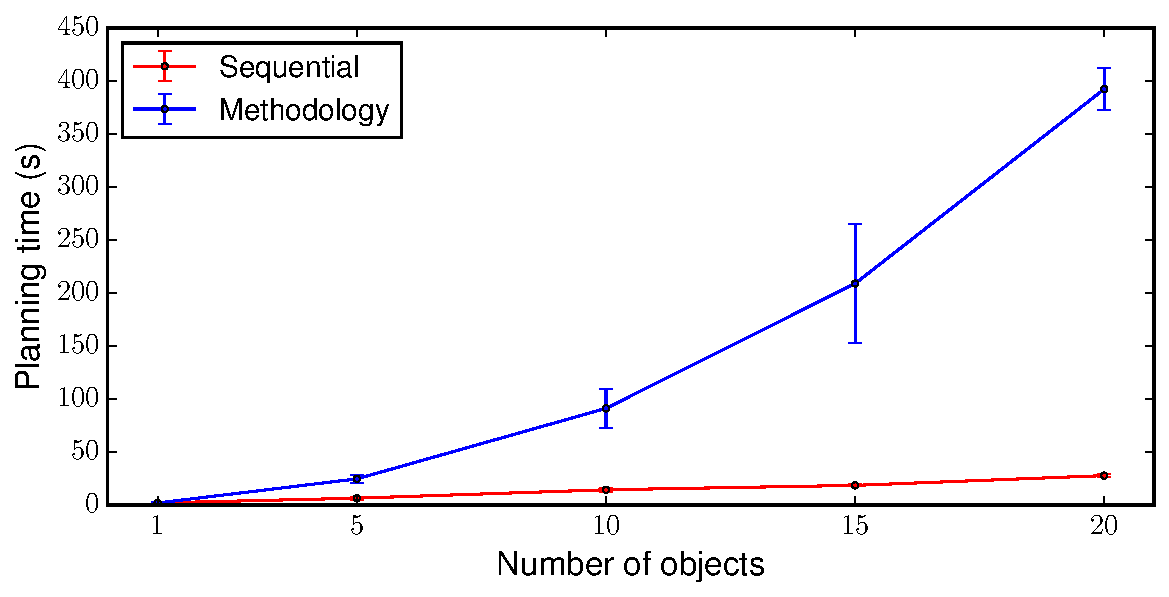
\includegraphics[width=0.9\textwidth]{imgs/experiment-time.pdf}
                % \caption*{Task Allocation Process}
            \end{figure}
        \end{block}
    }

    \frame{
        \frametitle{Experiments}

        \begin{block}{Traveled Distance}
            \begin{figure}[p]
                \centering
                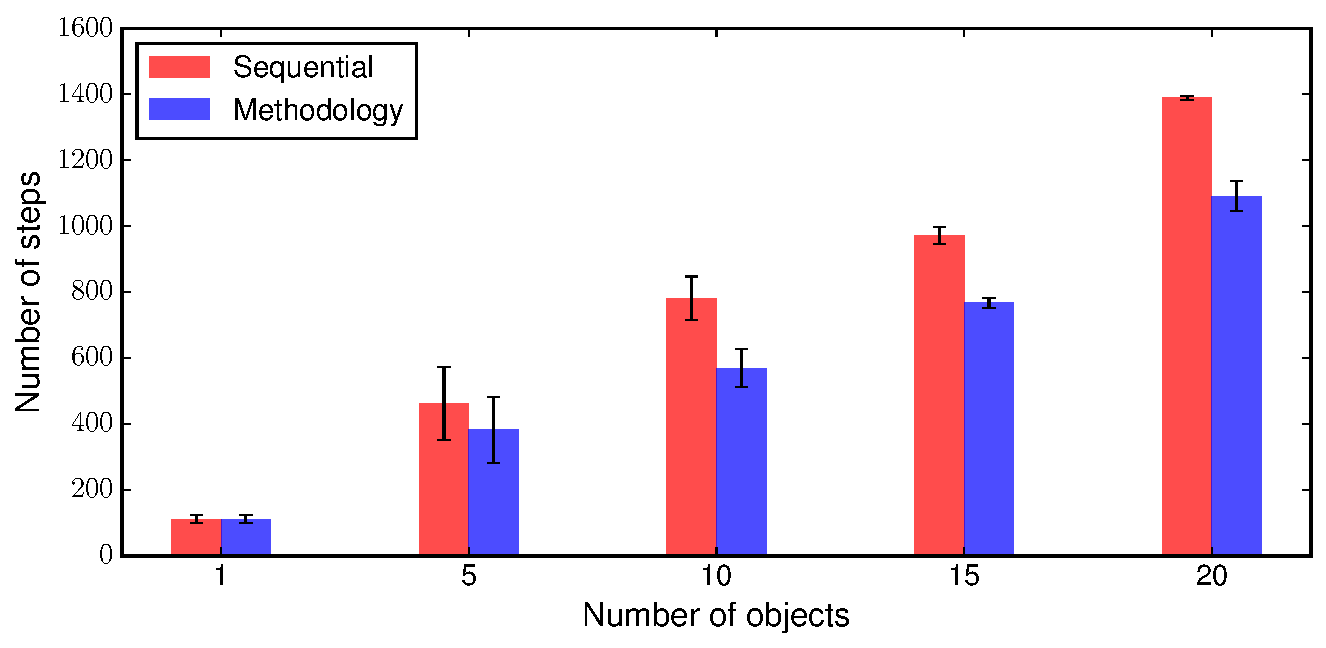
\includegraphics[width=0.9\textwidth]{imgs/experiment-move.pdf}
                % \caption*{Task Allocation Process}
            \end{figure}
        \end{block}
    }

    \section{Conclusion}

    \frame{
        \frametitle{Conclusion}

        This work proposes a methodology to efficiently execute the transportation of multiple objects in a environment with obstacles considering the use of a single robot.

        \vspace{0.2cm}
        The technique is capable of treat all aspects of the problem, starting from the path planning, task allocation and execution of the task.

        \vspace{0.2cm}
        The experiments showed the effectiveness of the method, presenting a improvement in relation to the total traveled distance by the robot when compared to a simple sequential method.

        \vspace{0.2cm}
        Future directions include the extension of the proposed process to consider a cooperative transport with multiple agents.
    }

    \section{Bibliografia} % (fold)
    \label{sec:bibliografia}

    \backupbegin
    \begin{frame}[allowframebreaks]
        \frametitle{References}

        \bibliographystyle{apalike}
        % \printbibliography
        \footnotesize
        \bibliography{references.bib}
    \end{frame}
    \backupend

\end{document}
